\documentclass{article}
\usepackage{listings}
\usepackage{color}
\usepackage{url}
\usepackage{graphicx}
\usepackage{titlesec}
\usepackage{wrapfig}
\usepackage{tabularx}

\setcounter{secnumdepth}{4}

\titleformat{\paragraph}
{\normalfont\normalsize\bfseries}{\theparagraph}{1em}{}
\titlespacing*{\paragraph}
{0pt}{3.25ex plus 1ex minus .2ex}{1.5ex plus .2ex}

% Define colors for syntax highlighting
\definecolor{codegreen}{rgb}{0,0.6,0}
\definecolor{codegray}{rgb}{0.5,0.5,0.5}
\definecolor{codepurple}{rgb}{0.58,0,0.82}
\definecolor{backcolour}{rgb}{0.95,0.95,0.92}

% Global settings
\lstset{
    backgroundcolor=\color{backcolour},   
    commentstyle=\color{codegreen},
    keywordstyle=\color{magenta},
    numberstyle=\tiny\color{codegray},
    stringstyle=\color{codepurple},
    basicstyle=\footnotesize\ttfamily,
    breakatwhitespace=false,         
    breaklines=true,                 
    captionpos=b,                    
    keepspaces=true,                 
    numbers=left,                    
    numbersep=5pt,                  
    showspaces=false,                
    showstringspaces=false,
    showtabs=false,                  
    tabsize=2
}

% Language-specific settings
\lstdefinestyle{Python}{
    language=Python,
    otherkeywords={self},             % Add keywords here
    morekeywords=[2]{True,False},     % Add built-in literals here
    keywordstyle=\color{blue},
    keywordstyle=[2]\color{codepurple}, % style for built-in literals
}

\lstdefinestyle{HTML}{
    language=HTML,
    tagstyle=\color{blue},
    usekeywordsintag=true,
    morekeywords={html, body, div, span}, % Add HTML tags here
}

\lstdefinestyle{CSS}{
    language=CSS,
    keywordstyle=\color{blue},
    morekeywords={margin, padding}, % Add CSS properties here
}

\lstdefinestyle{JavaScript}{
    language=JavaScript,
    keywordstyle=\color{blue},
    morekeywords={const, let, function}, % Add JavaScript keywords here
}

\title{Exercise Tracker Website \\ \vspace{10pt} \large Computer Science A-Level Project \normalsize}
\author{Marcus Ciobanu}
\date{}

\begin{document}

\maketitle
\newpage

\tableofcontents
\newpage

\section{Citations}
Listed in order of their appearance:
\begin{itemize}
  \item Statista (2022). UK fitness/health club market size 2021 | Statista. [online] Statista. Available at: \url{https://www.statista.com/statistics/1194831/fitness-health-club-market-size-uk/}.
\end{itemize}
\newpage

\section{Analysis}

\subsection{Define the Problem}
In recent years, the fitness industry has seen a boom in revenue and participation, with more people than ever being conscious of their health and diet. The figure below shows the market size of the gym, health \& fitness clubs industry in the United Kingdom (UK) from 2012 to 2022. As can be seen, there has been a steady increase up until 2020. 

Following this point, the COVID-19 pandemic caused a major blow to the gym industry. However, this is not representative of fitness as a whole. What the pandemic actually caused was a huge influx of beginners to fitness who, as a result of their abundance of free time and boredom, took up exercise. Furthermore, the figure also indicates a huge gain in market size from 2021 to 2022 as gyms opened back up. It can be expected that this trend will continue and the fitness industry’s market share will soar to new heights as those who began exercising during the pandemic purchase gym memberships.
\begin{figure}[ht]
  \raggedright
  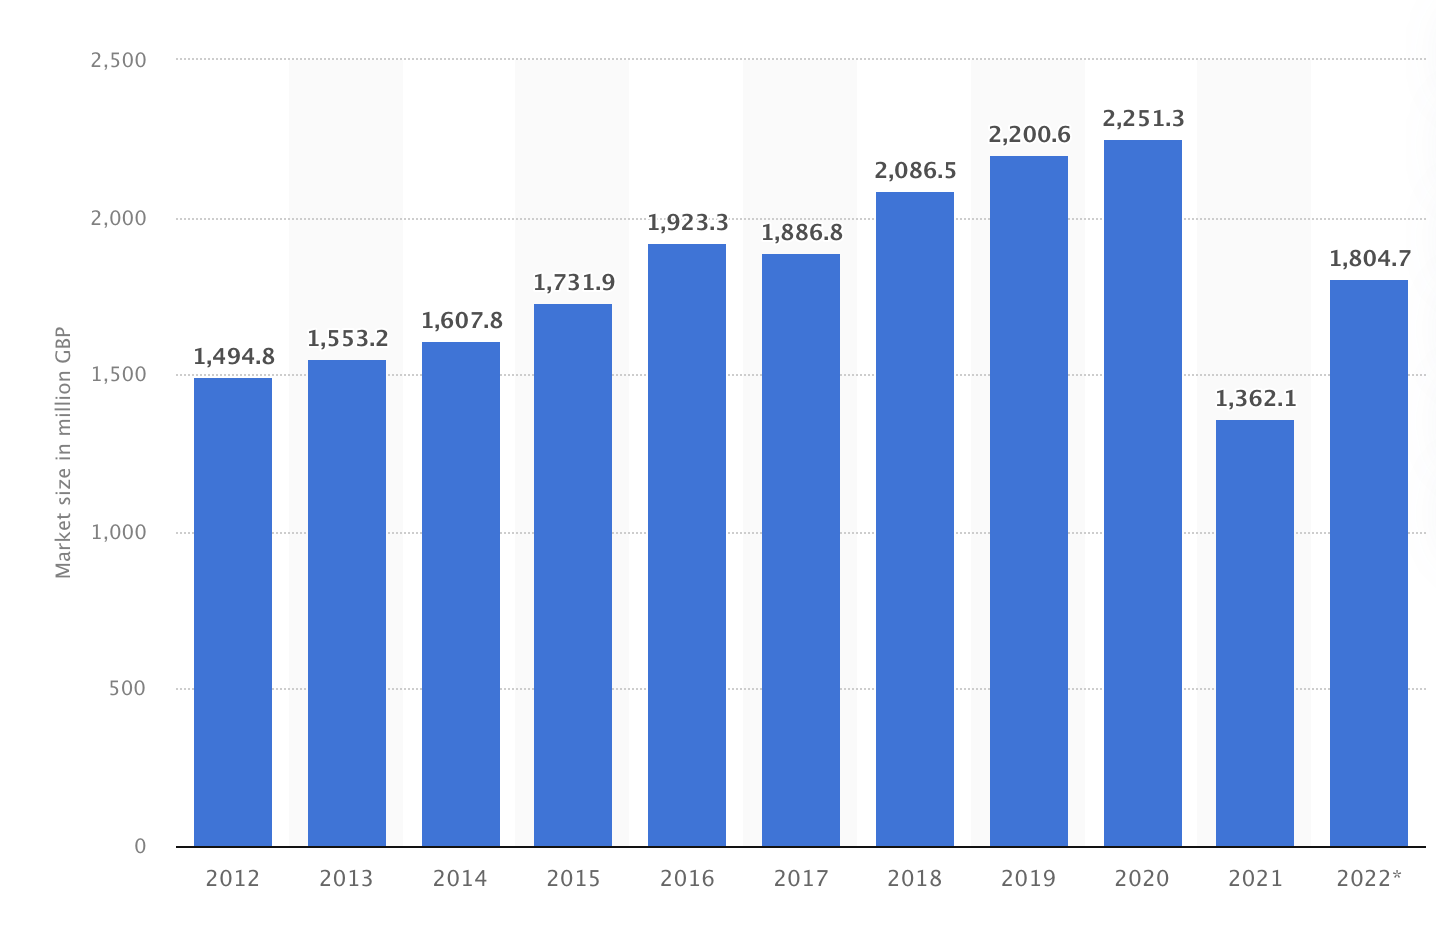
\includegraphics[width=1\textwidth]{Figure 1.png}
  \caption{Industry market size}
  \label{fig:Figure 1}
\end{figure}

As a result of the growth of the market, there is now room for competition in the digital fitness space(a previously monopolised industry where major players held the majority of the user base). New developments have the opportunity to seize user attention by solving their problems and capitalising on the unique needs of beginners.

From my own previous experience as a beginner in fitness, I can attest to the difficulty and friction associated with trying to record down everything manually. Having to carry a notebook and pen to every session is cumbersome and the formatting is often inconsistent. For the modern gym-goer, it is important to have a solution to this problem. The reason for tracking progress in the first place is that it is a critical element in optimising results to build muscle and/or lose weight. Rep ranges must be tracked and weight on the bar must be carefully monitored to maximise results for the minimum amount of effort. Evidently, such an endeavour is complex by nature, hence the need to make this as smooth and easy as possible for the beginner (lest they become demotivated and give up altogether). After all, if the experience is frictionless then you are more likely to record down all your workouts, leading to higher consistency and better results due to the compounding nature of incremental progress. 

In summary, there are more beginners than ever in fitness. Beginners suffer from a lack of knowledge regarding what to do. A simple solution that is easy and frictionless is required to help them track their activities and maximise progress. Therefore, my programming project involves developing an exercise tracking website that makes this process seamless and intuitive. 

\subsection{Why the Problem is suited to a Computational Solution}
Much of the suitability for this problem being suited to a computational solution stems from why this is a problem in the first place. Simply put, the analogue equivalent is massively inferior to any variation of a digital solution and makes it difficult for people to stick to it which harms progress. There are multiple reasons for this:
\begin{enumerate}
  \item As you advance, you will reach the point of having done hundreds of workouts. This results in thousands of exercises, tens of thousands of sets and hundreds of thousands of reps. Therefore, this large volume of data is best suited to being kept digitally, as it would result in many pages if done in analogue form.
  \item Pages are liable to physical damage such as being lost or set on fire, this is a risk as it could mean that you are unable to see what you have done previously or track your progress over an extended period of time. In contrast, data can be backed up on the cloud when done digitally, meaning it is kept safe.
  \item Handwriting can often be untidy and unclear and takes longer than typing or entering values into a database interface digitally. 
  \item Pages cannot be easily sorted through to gather meaningful insights (producing graphs for example) and could be sped up and made far more efficient through use of algorithms and computing power. 
  \item You do not need to bring a pen and paper to the gym with you if it is done digitally, as it can all be done on your phone which most people bring everywhere with them regardless. 
\end{enumerate}
\subsubsection{Computational methods that are appropriate}
As well as the reasons listed above that focus more on the comparison between the digital and analogue ways of solving the problem, there are also computational methods and constructs that lend themselves to the efficient and streamlined solving of the problem.
\paragraph{Thinking abstractly}
For in depth analysis and generation of insights from the data the user records such as producing graphs that display progress in a certain lift over time, abstraction can be used. The mechanisms behind the production of the graph are abstracted from the user for maximum ease of use and pure functionality. 

They would simply record their results into a GUI and select the option to produce a graph, much like how a programmer can input parameters into a function imported from a library. They know what it does and what is required to make it produce the results but do not and do not need to understand how it works. If we were to contrast this to the analogue equivalent, the user would need to understand how to plot graphs and translate data into the necessary formats. In this case, the use of abstraction not only lends itself to the computational solution but enhances it.
\paragraph{Thinking ahead}
Through the use of a computational solution, we can identify recurring scenarios and therefore develop functions that can be reused every time the user wants to carry out that task. For example, we know that if the user is using an exercise tracker they are going to want to record many workouts. Therefore, we can produce functions that take the expected inputs for these tasks (sets, reps, etc.) and produce outputs in a consistent, comparable format.
\newpage
\paragraph{Thinking procedurally}
\begin{wrapfigure}{l}{0.2\textwidth} % 'l' for left side, and width of the wrap
  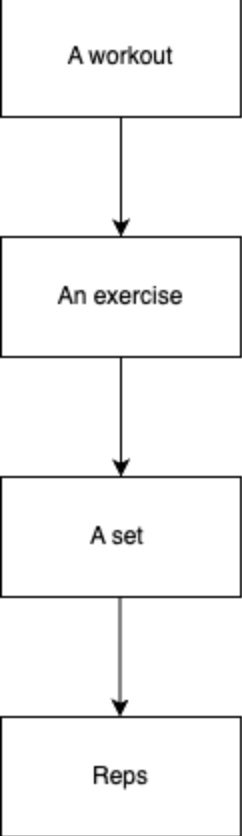
\includegraphics[width=0.2\textwidth]{Figure 2.png}
  \caption{Top-down design}
\end{wrapfigure}
When a user performs a workout, we understand that there will be a set ‘formula’ which they follow each time in a procedural manner. They would typically select an exercise, create a set then perform the reps that make up that set. Therefore, we can model this within the code through the use of a top-down design. 

As can be seen in the figure, we can break down the idea of a workout into nested modules of code in an order that the user would typically think of it in. These modules can then communicate with each other along the chain to produce the desired output. 

This method of top-design and decomposition is not only natural to the way of thinking of the user, but is also computationally efficient and speeds up the development process. It will also make the program far easier to maintain and test due to its modular nature. 

The modular nature also relates to thinking ahead, as it promotes code reusability and applying the same code to multiple iterations of the same scenario, further decreasing development time needed whilst ensuring consistent formatting and familiarity to the user. 

\subsection{Stakeholders}
Naturally, the primary group of stakeholders will be hobbyist gym goers, mostly due to the fact that they make up the majority of consumers in the market. Therefore, the website will be tailored to suit the needs of beginners to intermediates to maximise the usefulness to the average user. For example, all the exercises in the exercise database will include explanations on how to perform the exercise and what muscle groups it trains. Another example is the goal setting feature that will be included in the signup process which generates a recommended goal for them based on the information they enter during signup. Regardless, there will still be many features applicable to more advanced users as well, as the crossover is substantial and the core features of the website have utility throughout the spectrum of users.

The software is not intended for use by people under the age of 16, as this is the typical age requirement for most gyms and so it would be a poor use of resources and development time to make considerations for this user group. Despite this, the program is still usable by this group and there is no hard restriction in place to prevent them from using it. Simply put, it will not be designed in a way that places any priority on their specific needs and use cases, but they may be able to still use it for home workouts involving callisthenics and other bodyweight movements that do not require a gym to perform. 

In terms of people with disabilities, both mental and physical, the program retains its utility. Furthermore, no special features need be designed to cater for them. For anyone with physical disabilities, they can simply select the exercises that they can perform safely and to a good standard with their own disability in mind. Many exercises can be performed without the use of legs, for example dumbbell hammer curls. Therefore, in this case, the user will make their own adjustments so that the program can suit their needs. For anyone with mental disabilities, this should not have much impact on their ability to perform exercises, so the program should work as intended for them. However, the program will not cater for anyone with impaired vision, due to the difficulty of development of a comprehensive audio navigation system. This is a limitation, and restricts the user base for the project. 

Here is an example stakeholder to illustrate a typical use case:

\begin{figure}[ht]
  \centering
  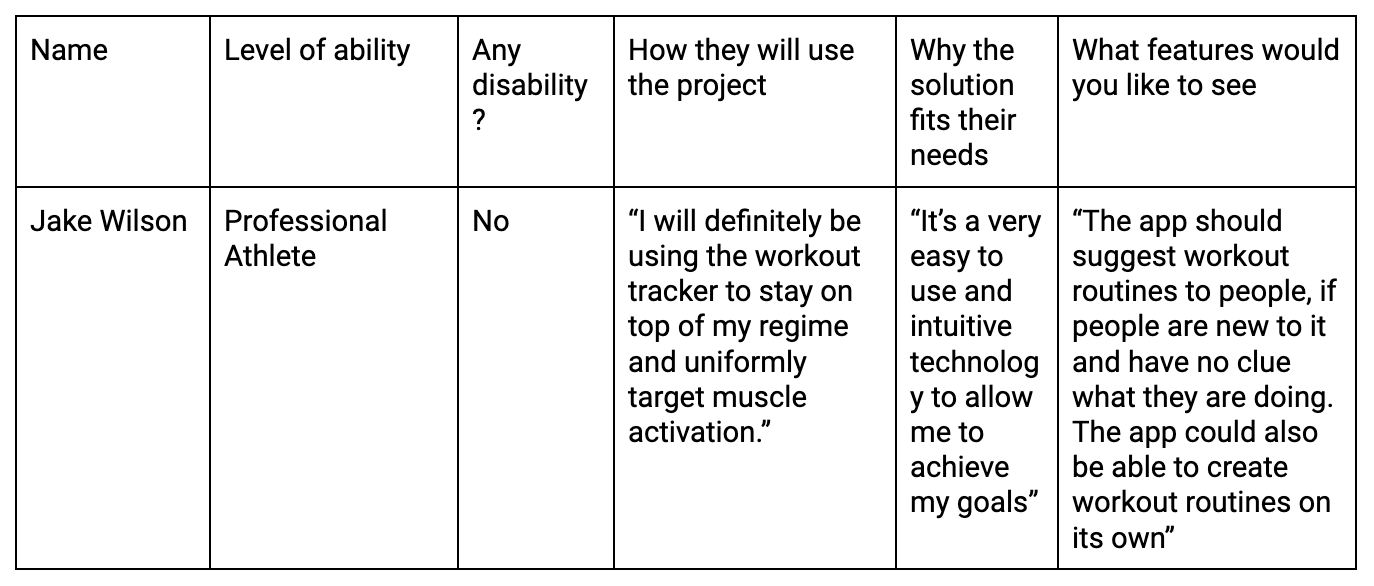
\includegraphics[width=1\textwidth]{Figure 3.png}
  \caption{Example stakeholder}
\end{figure}

Utilising feedback and requests from potential stakeholders such as Jake will be vital in ensuring that the finished project meets the needs and requirements of those who will be most likely to use it.

This iterative process of feedback and adjustment is important to increase customer satisfaction and widen the user base however it is also important to place limitations on what is realistic and achievable in the timeframe as what is just as important to stakeholders as a feature rich program is that the program is delivered on time and within budget. The balance between these two elements is something that will remain in mind throughout the whole project. 

\subsection{Research}

\subsubsection{Existing Systems}
There are two major existing systems that offer a workout tracking system similar to the proposed solution. These are Hevy and Strong. Alongside the research that follows, I have been a user of both programs at separate times for over a year so I believe this first-hand experience with both gives me the necessary insight to properly evaluate their features and identify the correct way to take on board this information for my own project. 

\paragraph{Hevy}
Hevy is the premier workout tracking app on the Android Play Store. The platform is different to the proposed solution (mobile vs. browser) but the core features remain the same and so it is valid to analyse. It incorporates workout tracking with a social media system where you can follow others and share your workouts and progress with a following. It works sort of like Instagram in that regard, being able to like and comment on others workouts. However, this element of the program is completely optional as you can make your account private, so for the purpose of this research, I will not be looking at this element of the program. It is also the cheaper of the 2 existing solutions priced at £2.99/month compared to Strong which is £4.69/month. 

\begin{figure}
  \centering
  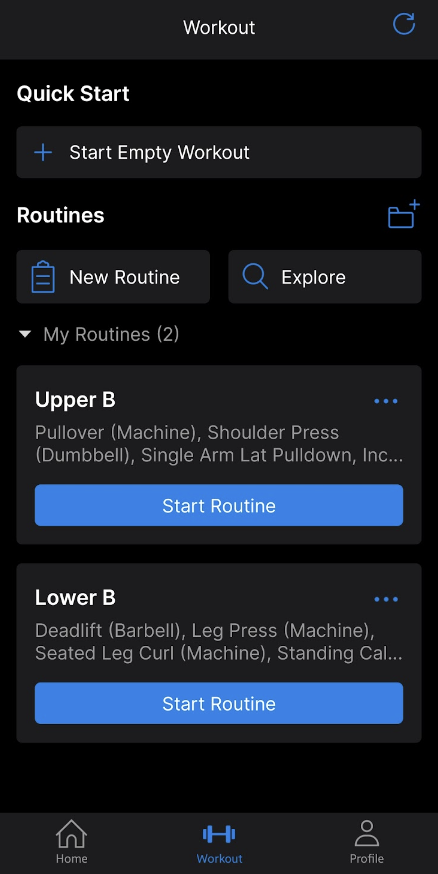
\includegraphics[width=0.4\textwidth]{Figure 4.png}
  \caption{Quick start page}
\end{figure}

The general consensus among users is that Hevy offers more features for analysis and tracking for a cheaper price whilst Strong offers a slick, clean UI with the actual workout tracking part of the app being very intuitive and easy to use. However, this is all subjective and in terms of user ratings, they both sit at a high 4 star rating with minimal criticism of either application.

In the surrounding pages are a few screenshots from my mobile phone from the app which illustrate a few key features that I will go through and evaluate. They cover a range of the app’s features from its workout tracking capabilities to its extensive section for analysis of progress and workouts. 

See Figure 4, the main section of the application which allows you to record your workouts. You can either create your own routines, choose from a range of templates in the explore section or select the quick start option. This will allow you to go straight into a workout and add your exercises on the fly. 

There is also an option to create routine folders. This allows increased organisation and to periodise your training into blocks sorted by folder (a useful feature for more advanced lifters who may want to alternate between load and deload periods). This could definitely be a feature to adopt in order to ensure that the program has adequate tailoring for all ability ranges. 

\begin{figure}
  \centering
  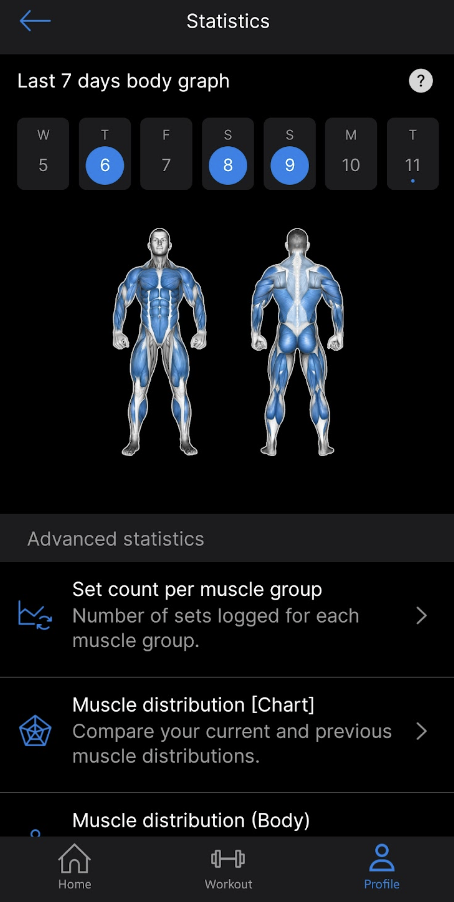
\includegraphics[width=0.4\textwidth]{Figure 5.png}
  \caption{Statistics page}
\end{figure}

Overall, Hevy does a great job of offering options for all use cases and ability levels, with customizability available if needed but not required. Furthermore, the UI is slick and intuitive, which is necessary for a small mobile screen.

The statistics section of the application is rather unique to Hevy, where you can analyse your progress in as much detail as you want to aid in organisation and planning. In particular, the heatmap is very useful, allowing you to see at a glance which muscle groups you have hit during that week. You can therefore quickly identify lacking muscles and pick exercises for your next workout that target them specifically. 

The advanced statistics section allows for a more indepth look at what the heatmap gives you at a glance. It logs sets per muscle group and shows a spider web chart of the distribution. All of these features can be leveraged for increased control and data on your progress. However, all of this is optional and doesn’t need to be used which is a good feature of
Hevy. It is as in depth and detailed as you want it to be.

\begin{figure}
  \centering
  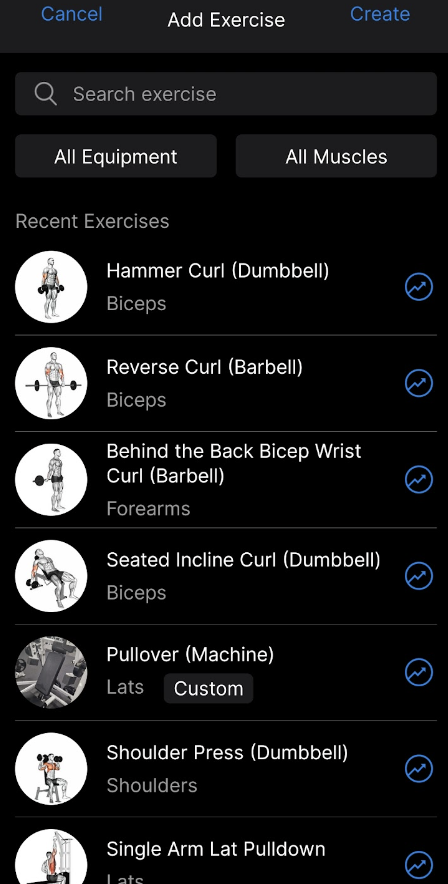
\includegraphics[width=0.4\textwidth]{Figure 6.png}
  \caption{Add exercise page}
\end{figure}

Figure 6 shows the exercise addition menu once you either start a routine or start empty exercise.

There is a large bank of premade exercises that cover nearly everything you will need. They also include an image and sometimes a video with instructions explaining how to perform every exercise. This is undoubtedly useful for beginners but more advanced lifters may want to do further research to optimise form and technique. 

All exercises when selected are automatically logged into a database, as well as the sets and reps you will go on to perform. 

As you can see further down the list, there is an exercise called ‘Pullover (Machine)’. This is a custom exercise. You can create your own exercises if your gym has some niche machinery or you wish to perform uncommon variations of certain exercises that cannot be found in the premade exercises. 

See Figure 7, this is the exercise creation menu. It can be accessed from the exercise addition menu by clicking on the button in the top right. 

You can create any exercise possible due to the features of the creation menu. A custom name and picture can be given. More importantly, the muscles it targets (both primary and secondary) are included, as well as the exercise type and equipment. This allows it to be included in the statistics section (heatmap, spiderweb) and also allows you to adjust weight and reps for progressive overload. 

\begin{figure}
  \centering
  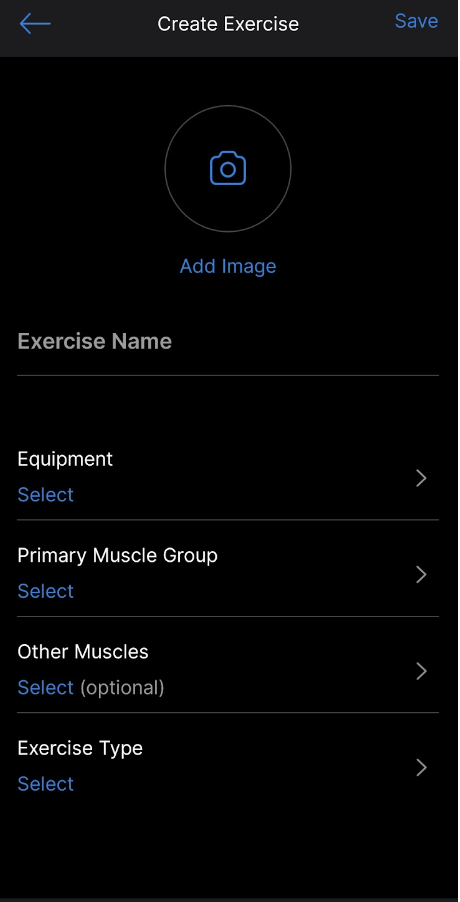
\includegraphics[width=0.4\textwidth]{Figure 7.png}
  \caption{Create exercise page}
\end{figure}

\newpage

This is absolutely an essential feature to add in my application as due to development time constraints, it will not be possible for me to create a comprehensive database of premade exercises. 


\paragraph{Strong}

There is a lot of carryover with the features from each app as they are very similar in a lot of ways. One difference I noticed was the far inferior statistics and analysis features that Strong offers in comparison to Hevy. There are only a few options on the profile tab to add charts that track workouts and exercise weight progressions over time. 

This information is rather surface level and doesn’t really provide much useful insight that would actually help you. Therefore, in my app, I would improve on this and make it more like Hevy. 

The profile system is also a lot less developed than Hevy. This makes sense, since Hevy also doubles as a fitness social media app in many ways, so Strong would have little reason to invest in such features. In my app, I would probably take a similar approach to Strong, as it will operate as a standalone package and users will not be able to interact with each other. 

\begin{figure}
  \centering
  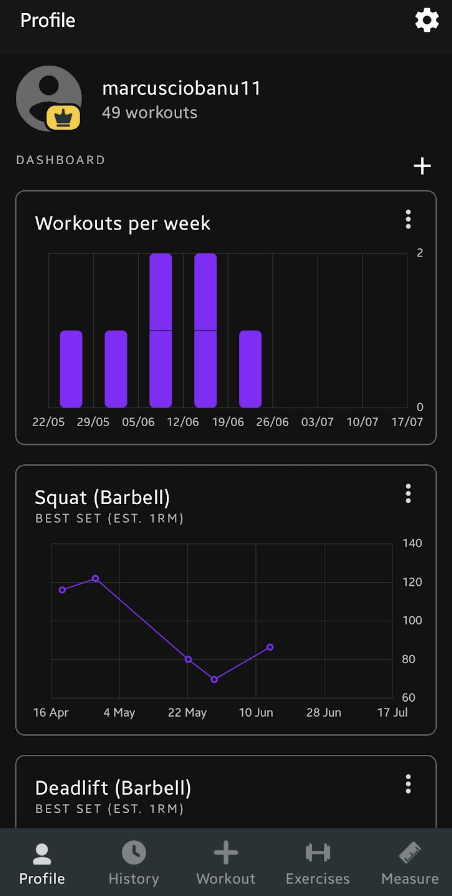
\includegraphics[width=0.4\textwidth]{Figure 8.png}
  \caption{Home page}
\end{figure}

The workout menu also functions in a very similar way to Hevy. However, the template system is far less developed, which is definitely something I would like to improve in my app. I found that the folder and stock template features were very useful so I would like to develop my app in that way. 

Despite this, all the other features are practically identical to Hevy. They function as intended and have utility. The base template of a workout tracker seems to be consistent no matter the developers which is a testament to its effectiveness. A quick start and template system will be integral to the workout tracking system in my application.

\begin{figure}
  \centering
  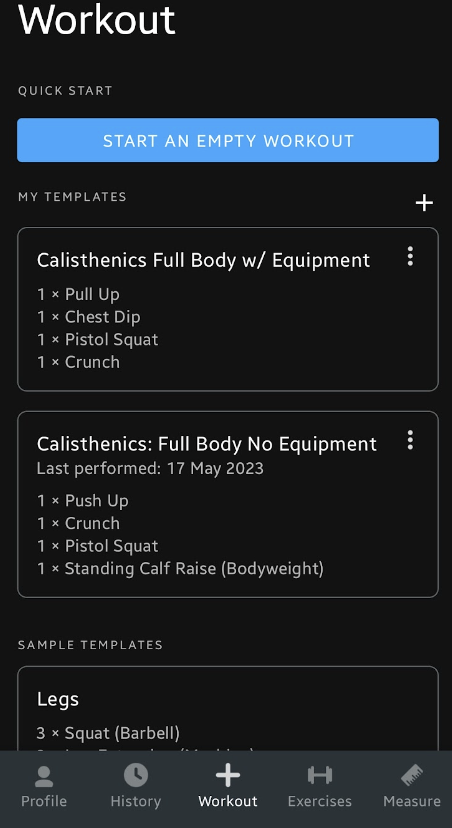
\includegraphics[width=0.4\textwidth]{Figure 9.png}
  \caption{Workout menu}
\end{figure}

The history menu is something that Hevy also has, but the layout in Strong is a lot more minimalist and focuses on showing the most important information. It is also categorised by month so it allows you to block and periodise your training which can certainly have utility for some people.

Overall, where Strong excels is its functional, intuitive and easy to use GUI. Especially for the mobile format, having little to no clutter is something that consumers would definitely appreciate and Strong has done that in a textbook manner. 

It is clear that despite the lack of updates and new features in Strong as compared to Hevy (the Strong developers have given up on the app in many ways), there is still a consistent user base and the reviews remain high. This is a testament to the strong foundation of the app within its core features. 

\paragraph{Summary of features to add}
\begin{itemize}
  \item Quick Start Workout Feature
  \begin{itemize}
    \item This will take the form of an interactive UI element that can be pressed
    \item This is necessary to further tailor my program to the beginner demographic who may not have a rigid routine and would appreciate the ability to start a workout and choose their exercises as they go along
  \end{itemize}
  \item Folder Organisation System
  \begin{itemize}
    \item This will be a niche feature with high utility to ensure that the program also retains good use for more advanced users who may have periodisation blocking and alternate their training regimes.
  \end{itemize} 
  \item Exercise Creation Function
  \begin{itemize}
    \item Essential feature to reduce development and make it so that users can record their workouts no matter the equipment they use or the gym they go to
    \item This will be implemented as its own page that is linked through the workout tracking section.
  \end{itemize}
  \item Statistics Section
  \begin{itemize}
    \item Great feature for both beginners and advanced users alike as it is as detailed and informative as you want it to be and gives useful information to see if you are on the right track
    \item This will have its own dedicated section on the website with multiple pages 
  \end{itemize}
\end{itemize}

\subsubsection{Features of proposed solution}

Key features: 
\begin{itemize}
  \item A workout tracking section with a quick start option and a template creation and selection module with a folder organisation section for training blocking and periodisation
  \item A statistics/analysis section where users can see their muscle group distribution by sets, reps or weight. There should also be graphs to track progressive overload over time. 
  \item A workout history section with a scroll down menu to view all past workouts and the key information from each workout 
\end{itemize}

The listed features above are the most important because they provide the maximum amount of utility to the user. There are many more features I will likely add, but these remain a priority as they are essential to ensuring the program meets the needs of the stakeholders. That being, it is easy to use and intuitive whilst providing useful insight to maximise progress with minimal effort.

\subsubsection{Limitations}

\begin{enumerate}
  \item There will be no user to user connection like Hevy has. In other words, there will be no follow, posting or liking systems and you cannot see the progress of friends etc. This is due to development time constraints.
  \item I will not be able to port this website to mobile formats, so when a mobile browser loads the web app, they will be faced with the desktop layout. This may prove cumbersome for users, but since I am developing on desktop it would make development far easier. Therefore, I will not provide a mobile reformatting again due to time constraints. 
  \item Testing will be limited to desktop. This means that there may be undiscovered bugs that arise when the website is opened on mobile. This, combined with the poor mobile formatting, will make the user experience for this demographic poor, but it is necessary to ensure that the solution is completed on time with the necessary features. 
\end{enumerate}

\subsubsection{Measurable criteria}

\begin{figure}
  \centering
  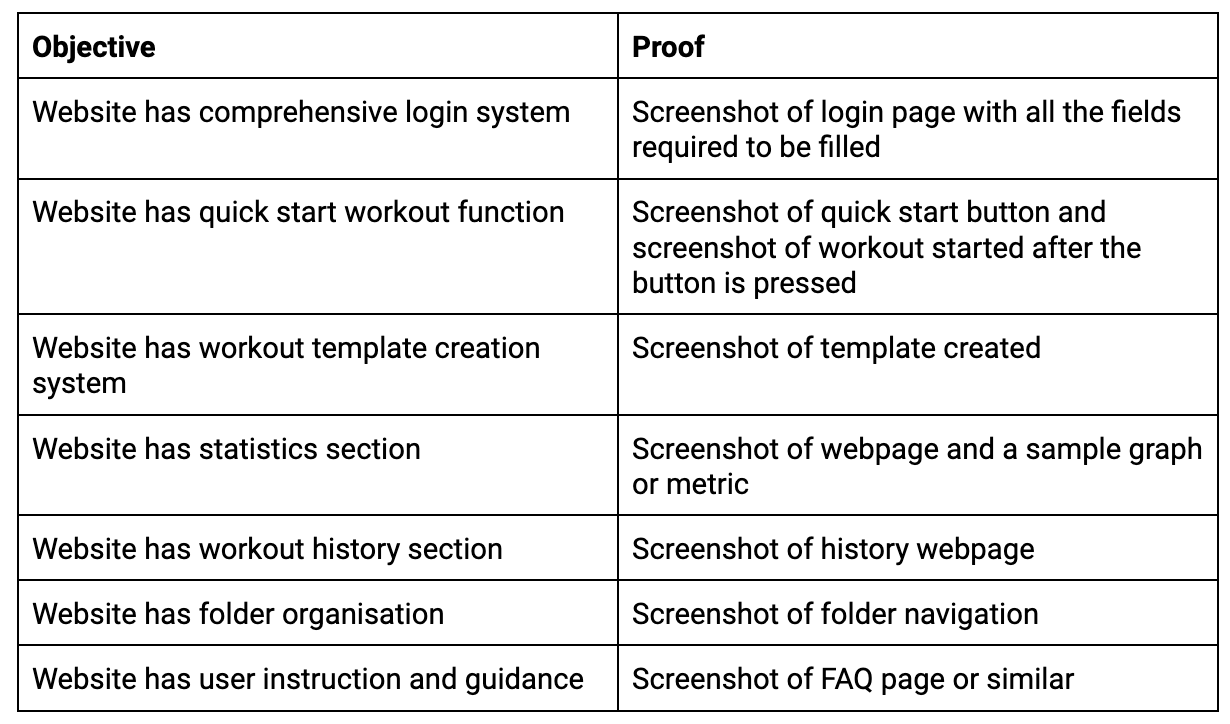
\includegraphics[width=1\textwidth]{Figure 10.png}
  \caption{Measurable criteria}
\end{figure}

\newpage

\subsubsection{Solution requirements}

\begin{itemize}
  \item Users must create or login to an account upon opening website
  \begin{itemize}
    \item Account creation details:
    \begin{itemize}
      \item Name (full)
      \item Username
      \item Email
      \item Password
    \end{itemize}
  \end{itemize}
  \item Users should be able to track and record workouts
  \begin{itemize}
    \item Start a workout by template or quick start
    \item Add exercises (either from the premade database or custom)
    \item Add sets
    \item Add reps 
    \item Specify type of set (drop set, failure set, warm up set, working set)
    \item Be able to view all past workouts
  \end{itemize}
\end{itemize}

These are the core features that will make the web app work, but there are many quality of life features that I will also plan to add. This outlines the bare minimum for it to function as intended with some essential features. Everything else only improves on the user experience in essence. 

In terms of hardware requirements, the device the user is currently on must be able to run a web browser and connect to the internet. They must also have around 1GB of local storage available to leave plenty room for database downloads and caching websites locally.

\section{Design}
\end{document}